\documentclass[11pt,letterpaper]{article}
\pdfoutput=1

\usepackage{mycommands1,amssymb,amsmath,amsthm,color,pagesize,outlines,cite,subfigure,epsfig}
\usepackage[small]{caption}
\usepackage{hyperref} % for linking references
\hypersetup{colorlinks = true, citecolor = blue, urlcolor = blue}

\usepackage{stackrel}

\usepackage[round]{natbib}

% for algorithm
%\usepackage[noend]{algpseudocode}
%\usepackage{algorithm}

% DON'T change margins - should be 1 inch all around.
\addtolength{\evensidemargin}{-.5in}
\addtolength{\oddsidemargin}{-.5in}
\addtolength{\textwidth}{0.9in}
\addtolength{\textheight}{0.9in}
\addtolength{\topmargin}{-.4in}

%% measurements for 1 inch margin
%\addtolength{\oddsidemargin}{-.875in}
%\addtolength{\evensidemargin}{-.875in}
%\addtolength{\textwidth}{1.75in}
%\addtolength{\topmargin}{-.875in}
%\addtolength{\textheight}{1.75in}

%\pagestyle{myheadings}
%\markboth{}{\underline{{\bf Notes: (do not circulate)} \hspace{4.5cm} {\sc  Ansu Chatterjee} \hspace{0.25cm}}}

\DeclareMathOperator*{\ve}{vec}
\DeclareMathOperator*{\diag}{diag }
\DeclareMathOperator*{\supp}{supp }
\DeclareMathOperator*{\Tr}{Tr}
\DeclareMathOperator*{\argmin}{arg\,min}
\DeclareMathOperator*{\argmax}{arg\,max}
\DeclareMathOperator*{\Th}{^{\text{th}}}
\DeclareMathOperator*{\kl}{\text{KL}}
\DeclareMathOperator*{\rtbd}{{\colrbf tbd}}

\makeatletter
\newcommand{\opnorm}{\@ifstar\@opnorms\@opnorm}
\newcommand{\@opnorms}[1]{%
  \left|\mkern-1.5mu\left|\mkern-1.5mu\left|
   #1
  \right|\mkern-1.5mu\right|\mkern-1.5mu\right|
}
\newcommand{\@opnorm}[2][]{%
  \mathopen{#1|\mkern-1.5mu#1|\mkern-1.5mu#1|}
  #2
  \mathclose{#1|\mkern-1.5mu#1|\mkern-1.5mu#1|}
}
\makeatother

%% Appendix theorem counter
\usepackage{chngcntr}
\usepackage{apptools}
\AtAppendix{\counterwithin{Theorem}{section}}
\numberwithin{equation}{section}

\begin{document}

\newtheorem{Theorem}{Theorem}[section]
\newtheorem{Lemma}[Theorem]{Lemma}
\newtheorem{Corollary}[Theorem]{Corollary}
\newtheorem{Proposition}[Theorem]{Proposition}
\newtheorem{Conjecture}[Theorem]{Conjecture}
\theoremstyle{definition} \newtheorem{Definition}[Theorem]{Definition}
\newtheorem{Example}{Example}[section]
\newtheorem{Algorithm}{Algorithm}
\newtheorem{Remark}{Remark}

\title{Title}
\date{}
%\author{
%	Subhabrata Majumdar\thanks{Email: {\tt smajumdar@ufl.edu}}\\
%	and\\
%	George Michailidis\thanks{Corresponding author. Email: {\tt gmichail@ufl.edu}}\\
%	University of Florida, Gainesville, FL, USA
%}
\maketitle

\noindent\textbf{Abstract}: 

\vspace{.5cm}
\noindent\textbf{Keywords}:
%\newpage

\section{Formulation}
Consider a random variable $\BX \in \BR^p$ that has a sparse dependency structure among its features. This graph structure is potentially non-linear, and we want to infer the structure from a data matrix $\bfX \in \BM(n,p)$.

We assume a multi-layer generative model for the structure:
%
\begin{align*}
\bfX &= \varphi (\bfH_1) \bfB_1 + \bfE_x; \quad \BE \sim \cN_p ({\bf 0}, \Sigma_x),\\
\bfH_1 &= \varphi (\bfH_2) \bfB_2 + \bfF_1; \quad \BF_1 \sim \cN_{p_1} ({\bf 0}, \Sigma_1),\\
\cdots\\
\bfH_{L-1} &=
\varphi (\bfH_L) \bfB_L + \bfF_{L-1}; \quad \BF_{L-1} \sim \cN_{p_{L-1}} ({\bf 0}, \Sigma_{L-1}),\\
\BH_L & \sim \cN_{p_L} ({\bf 0}, \Sigma_L).
\end{align*}
%
with $L$ hidden layers, and $\varphi(\cdot)$ being a pointwise known transformation (e.g. ReLU, sigmoid, tanh).
When $\Sigma_x$ and $\Sigma_l, l \in \cI_L$ are diagonal, it is the Non-linear Gaussian Belief Network of \cite{FreyHinton99}. In our case, we keep $\Sigma_x$ non-diagonal (but sparse), while others diagonal.

The negative log-likelihood function is
%
\begin{align*}
-\ell( \bfX| \cH, \cB, \Omega) &= \frac{n}{2}\left[ \Tr \left(\bfS_x \Omega_x \right) - \log \det \Omega_x +
\sum_{l=1}^L \left\{ \Tr \left(\bfS_l \Omega_l \right) - \log \det \Omega_l \right\} \right]
\end{align*}
%
where $\bfS_x = \bfE_x^T \bfE_x/n, \bfS_l = \bfF_l^T \bfF_l/n$ for $l = 1, \ldots, L-1$ and $\bfS_L = \bfH_L^T \bfH_L/n$.
%
Inferring the distribution of the hidden variables is difficult so we assume pointwise variational approximations:
%
$$ h_{ij,l} \sim N(\mu_{ijl}, s_{ijl}); \quad i \in \cI_n, j \in \cI_{p_l}, l \in \cI_L. $$
%
Collect the variational parameters in $\cM := \{ \bfM_1, \ldots, \bfM_L\}, \cS:= \{ \bfS_1, \ldots, \bfS_L\}$. Now we have the variational lower-bound
%
\begin{align}\label{eqn:elbo}
\ell( \bfX| \cH, \cB, \Omega) \geq
\BE_q \ell (\bfX,\cH| \cB,\Omega,\cM,\cS) - \BE_q \log q(\cH| \bfX, \cB,\Omega,\cM,\cS)
\end{align}
%
Denote this lower bound by $\ell_q(\bfX|\cB,\Omega,\cM,\cS)$. Under the simplified model $\Sigma_l = \bfsigma_l \bfI$ for $l \in \cI_L$, the second term becomes \citep{FreyHinton99}
%
\begin{align}\label{eqn:KLdivergence}
\BE_q \log q(\cH| \bfX, \cB,\Omega,\cM,\cS) = \frac{1}{2} \left[\sum_{i=1}^n \sum_{j=1}^{p_l} \sum_{l=1}^L \log \frac{s_{ijl}}{\sigma_{jl}} -\frac{s_{ijl}}{\sigma_{jl}} + n \log \det \Omega_x + \text{constant} \right].
\end{align}
%
For the first term we have
%
\begin{align*}
\BE_q \ell (\bfX,\cH| \cB,\Omega,\cM,\cS) &=
\frac{n}{2} \BE_q \left[ \Tr ( \bfS_x \Omega_x) + \sum_{l=1}^L \Tr(\bfS_l \Omega_l) \right]\\
&= 
\end{align*}
%
which simplifies to \citep{FreyHinton99}
%
\begin{align}\label{eqn:loglik}
- \left[ \BE_q \Tr(\bfE_x^T \bfE_x \Omega_x)  +
\sum_{i=1}^n \sum_{j=1}^{p_l} \sum_{l=1}^{L-1}
\frac{1}{\sigma_{jl}} \left\{ (\mu_{ijl} - b_{ij,l+1} m_{ij,l+1})^2 + b_{ij,l+1}^2 v_{ij,l+1} \right\} + \text{const} \right]
\end{align}
% last layer expectation is constant
%
where $m_{ijl} = \BE_q \varphi( h_{ijl}), v_{ijl} = \BE_q (\varphi( h_{ijl}) - m_{ijl})^2$.

\subsection{Objective function}
Our goal is to solve a penalized version of the variational lower bound in \eqref{eqn:elbo}:
%
\begin{align*}
-\frac{2}{n} \ell_q(\bfX|\cB,\Omega,\cM,\cS) + \sum_{l=1}^L
\lambda_{nl} \| \bfB_l\|_1 +\gamma_n  \| \Omega_x \|_{1,\text{off}}
\end{align*}
%

We take the greedy strategy of solving two-layer problems successively. This means molte-carlo {\it sequential} EM: first solve for the variational parameters $(\bfM_1, \bfS_1) = ((\mu_{ij,1}, s_{ij,1}))$, in the E step, then solve for $(\bfB_1,\Omega_x)$ in the M step, and continue until convergence. After convergence is reached, go to the next layer. Similar to \cite{Hinton06, Bengio07}. 

%We assume a rank-1 representation for $\bfM \equiv \bfM_1$ and $\bfS \equiv \bfS_1$:
%\begin{align*}
%\bfM &= \bfa \bfb^T, \bfa \in \BR^n, \bfb \in \BR^q, q \equiv p_1,\\
%\bfS &= \bfc \bfd^T, \bfc \in \BR^n, \bfd \in \BR^q
%\end{align*}
%%
%We further assume generative parameters for $\bfa$: $a_i \sim N(\mu,\sigma^2)$ for $i \in \cI_n$.

\begin{figure}[t]
\centering
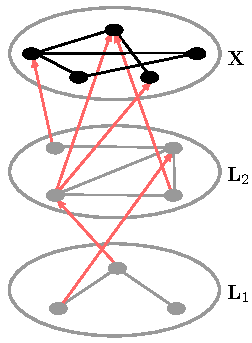
\includegraphics[height=.2\textheight]{latentmultilayer}
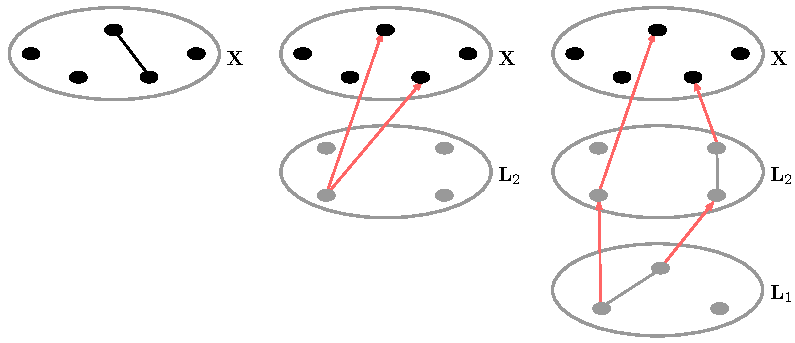
\includegraphics[height=.2\textheight]{latentinteractions}
\end{figure}

The objective function for a two-layer model, with the top layer being the observed data $\cX$, is:
%
\begin{align*}
&\Tr \left[ \frac{1}{n} (\bfX - \varphi(\bfH) \bfB )^T (\bfX - \varphi(\bfH) \bfB ) \Omega_x \right] + 
\log \det \Omega_x + \lambda_n \| \bfB\|_1 +
\gamma_n \| \Omega_x \|_{1,\text{off}}.\\
\end{align*}
%
When $\varphi$ is identity, this becomes a sparse factor model (refs). However for non-linear $\varphi$ optimizing this becomes difficult. To tackle this, we use a variational approximation of the objective function. We assume the following hierarchical generative model for the hidden variables and associated variational parameters:
%
\begin{align}
h_{ij} & \sim N(\mu_{ij}, \sigma_{ij}^2), \notag\\
\mu_{ij} & \sim \sum_{k=1}^K I_{mk} N(\mu_{mk}, \sigma_{mk}^2); \quad I_{mk} = \text{Ber}(\pi_{mk}) \notag\\
\log \sigma_{ij} & \sim \sum_{k=1}^K I_{sk} N(\mu_{sk}, \sigma_{sk}^2); \quad I_{sk} = \text{Ber}(\pi_{sk}). \label{eqn:hierarchy}
\end{align}
%
Thus in total there are $6K$ generative parameters. Following the framework of hierarchical variational models (refs), we replace the negative loglikelihood $-l (\bfx; \theta)$ by a hierarchical evidence lower bound (HELBO) $-\bar l (\bfx; \bfvt)$, defined as:
%
$$
\bar l(\bfx; \bfeta) = \BE_2 l(\bfx, \bfh_\varphi; \bfeta) +
\BE_1 \text{KL}(q(\bfm, \bfs| \bfx)\| p(\bfm, \bfs)) +
\text{KL} (q(\bfvt| \bfz) \|  p(\bfvt)),
$$
%
with $\BE_1$ and $\BE_2$ denoting expectations over the distributions of $(\bfm, \bfs)$ only and both the latent data and variational parameter distributions, respectively. Our desired set of parameter estimates (variational as well as generative) are defined as the minimizer of a penalized version of this HELBO:
%
\begin{align}\label{eqn:ObjFun}
\hat \bfeta = \argmin_\bfeta \left[ \frac{1}{n} \sum_{i=1}^n
\bar l(\bfx_i; \bfeta) + \lambda_n \| \bfB\|_1 +
\gamma_n \| \Omega_x \|_{1,\text{off}} \right].
\end{align}

\subsection{Computational algorithm}
Our objective function in \eqref{eqn:ObjFun} is not convex in general. However, with the variational specifications in \eqref{eqn:hierarchy} it is bi-convex with respect to the variational and generative components of our parameter vector.

\begin{Proposition}\label{prop:biconvex}
The objective function in \eqref{eqn:ObjFun} is bi-convex with respect to the variational parameters $\bfvt$ and generative parameters $\bftheta$.
\end{Proposition}

\paragraph{E-step:} we solve for the variational parameters by minimizing the following (take $\bfH_\varphi \equiv \varphi(\bfH)$)
%
\begin{align*}
\cF(\bfM, \bfS) &= \BE_q \Tr \left[ \frac{1}{n} (\bfX - \bfH_\varphi \bfB )^T (\bfX - \bfH_\varphi \bfB ) \Omega_x \right]\\
&= \Tr \left[ \left\{ \frac{1}{n} (\bfX - \bfM_\varphi \bfB )^T(\bfX - \bfM_\varphi \bfB ) +
\bfB^T \bfV_\varphi \bfB \right\} \Omega_x \right]\\
&= \left[ \sum_{j=1}^p \sum_{j'=1}^p \omega_{jj'} \left\{
\frac{1}{n} (\bfX_j - \bfM_\varphi \bfB_j)^T (\bfX_{j'} - \bfM_\varphi \bfB_{j'}) + \bfB_j^T \bfV_\varphi \bfB_{j'}
\right\}\right]\\
&= \sum_{j,j'=1}^p \omega_{jj'} \left\{
-\frac{2}{n} \bfX_j^T \bfM_\varphi \bfB_{j'} + \bfB_j^T \left( \frac{1}{n} \bfM_\varphi^T \bfM_\varphi + \bfV_\varphi \right) \bfB_{j'}\right\} + c
\end{align*}
%
%% variance term will be Eq ((phi(H)-M_phi)^T (phi(H)-M_phi))
where $(\bfM_\varphi)_{ik} = \BE_q \varphi (h_{ik})$ for $i \in \cI_n, k \in \cI_q$, and $\bfV_\varphi = \BE_q [(\bfH_\varphi - \bfM_\varphi)^T (\bfH_\varphi - \bfM_\varphi)/n]$. Differentiating with respect to entries of $\bfM$ we now have
%
\begin{align*}
\frac{\partial \cF}{\partial \mu_{ik}} = \sum_{j,j'=1}^p \omega_{jj'} \left[
-\frac{2}{n} x_{ij} \frac{d m_{ik}}{d \mu_{ik}} b_{j'k} +
\frac{1}{n} \left\{ 2 b_{jk} \left( 2 m_{ik} + \sum_{i' \neq i} m_{i'k} \right) \frac{dm_{ik}}{d\mu_{ik}} b_{j'k} \right\} +
{\colrbf tbd}
\right]
\end{align*}
%
Using chain rule, we get the derivatives with respect to the component vectors:
%
$$
\frac{\partial \cF}{\partial \mu} = \bfb^T \frac{\partial \cF}{\partial (\mu \bfb)}; \quad
\frac{\partial \cF}{\partial \sigma} = {\colrbf tbd}; \quad
\frac{\partial \cF}{\partial b_k} = \bfa^T \frac{\partial \cF}{\partial (b_k \bfa)}.
$$

\paragraph{M-step:} First generate data $\bfH_\varphi$ using the variational parameters $(\bfM, \bfS)$. Then obtain $\bfB,\Omega_x$ by solving a penalized LS  problem:
%
$$
\{ \hat \bfB, \hat \Omega_x \} = \argmin_{\bfB,\Omega_x} \Tr(\bfS^\varphi_x \Omega_x) + \log \det \Omega_x + \| \bfB \|_1 + \| \Omega_x \|_{\text{off},1}.
$$
%

\section{Theoretical properties}

\subsection{Concentration bounds for a two-layer model}
Define equivalence classes, $\bftheta = \ve (\bfB, \Omega_{x,\text{off}})$, $\bfvt$ denoting the variational parameters, $\bfeta = (\bftheta, \bfvt)$. Then we are minimizing
%
$$
\BE_q \left[ l(\bfx; \bfz, \bfeta) + \kl(q(\bfz| \bfvt_1) \| p(\bfz)) +
\kl( r(\bfvt_1| \bfz; \bfvt) \| q(\bfvt_1; \bfvt)) \right] + P( \bftheta ).
$$
%
define the negative hierarchical ELBO by $\bar l(\cdot)$. We consider a $\ell_1$-penalty
%
$$ P(\bftheta) = \rho_1 \| \bfbeta \|_1 + \rho_2 \| \bfomega \|_1 = \lambda P_\alpha (\bftheta) $$
%
by reparameterizing the penalties: $ \lambda = \rho_1 + \rho_2, \alpha = \rho_1/\lambda$.

Conditions 1, 2, 3 same as those in SPINN paper.

Define $V_n(\bfeta) = \BE \bar l(\bfx; \bfeta) - \bar l(\bfX; \bfeta)$, $\cE(\bfeta|\bfeta_0), \bar \cE(\bfeta|\bfeta_0)$ as in \cite{StadlerEtal10}.

\begin{Theorem}\label{thm:thm1}
Define the event
%
$$
\cT = \left\{ \cX: \sup_\bfeta \frac{ |V_n(\bfeta_0^\bfeta) - V_n(\bfeta)| }{\lambda_0 \vee
(P_\alpha(\bftheta - \bftheta_0^\bfeta) + \| \bfvt - \bfvt_0^\bfeta \|_2) }
\leq T \lambda_0 \right\}
$$
%
for $T \geq 1, \lambda_0 > 0$. Then for the solution $\hat \bfeta$ defined in $\rtbd$ that is calculated using a fixed sample $\cX \in \cT$, we have
%
$$
\cE(\hat \bfeta ) + \frac{\lambda - 2T\lambda_0}{2} \| \hat \bftheta_{S^c} \|_1 \leq
\left[ (\lambda + 2T\lambda_0) (\alpha \sqrt{s_\beta} + (1-\alpha) \sqrt{s_\omega}) c_0 \right]^2
$$
%
for some constant $c_0 > 0$.
\end{Theorem}

\paragraph{Condition 4.} The gradient of $\bar l(\cdot)$ with respect to the model parameters is bounded above:
%
$$
\left\| \nabla_\bfeta \bar l(\bfx; \bfeta) \right\|_\infty \leq G(\bfx)
$$
%
for some function $G: \BR^p \mapsto \BR^+$. Further, there exists $c' > 0$ such that
%
$$
| \bar l(\bfx; \bfeta) - \bar l(\bfx, \bfeta')| \BI(G(\bfx) \leq M)) \leq c'
$$
%
for any $M \geq 0$ and $\bfeta, \bfeta'$.

\begin{Theorem}\label{thm:thm2}
For the choice of $\lambda_0$:
%
\begin{align}\label{eqn:thm2st1}
\lambda_0 = (20 + c_1 )^{1/2} \frac{\log n}{\sqrt n} \left[ \frac{ \sqrt{2 c_2 K}}{m_\alpha} + 
\log \left( \frac{n \sqrt{c_2 K} \log n}{m_\alpha} \right) \sqrt{ \log (2d)} \right],
\end{align}
%
and any $T \geq 1$, the event $\cT$ happens with probability $\geq$
%
\begin{align}\label{eqn:thm2st2}
1 - c_3 \log n \exp \left[ - \frac{n T^2 \lambda_0^2 }{ c_4^2 K \log n} \right] - \frac{c_5 \sqrt K}{n^{3/2} \log n},
\end{align}
%
for some constants $c_1, c_2, c_3, c_4, c_5 > 0$, and sample size condition $n \log n \geq m_\alpha (c_2 K)^{-1/2}$.
\end{Theorem}

Using theorems \ref{thm:thm1} and \ref{thm:thm2} a concentration bound on both the excess risk and weights of irrelevant nodes is now immediate.

\begin{Corollary}\label{corollary:cor1}
Suppose conditions 1-4 are satisfied, and we have sample size $n$ so that $n \log n \geq m_\alpha (c_2 K)^{-1/2}$. Then for random $\cX$ and $\lambda_n \geq 2 \lambda_0$, with $\lambda_0$ defined as \eqref{eqn:thm2st1}, we have
$$
\cE(\hat \bfeta ) + \frac{\lambda_n - 2\lambda_0}{2} \| \hat \bftheta_{S^c} \|_1 \leq
c_0^2 m_\alpha^2 (\lambda_n + 2\lambda_0)^2 s
$$
%
with probability larger than or equal to
%
$$
1 - c_3 \log n \exp \left[ - \frac{n \lambda_0^2 }{ c_4^2 K \log n} \right] - \frac{c_5 \sqrt K}{n^{3/2} \log n}.
$$
%
\end{Corollary}

\subsection{Multi-layer sparse latent model}


\section{Proofs of main results}

\begin{proof}[Proof of Proposition~\ref{prop:biconvex}]
Since our penalties are convex, we only need to prove the biconvexity of the HELBO. For this we first simplify its squared error part. For $j,j' \in \cI_p$, consider $\bfX_j$ to be the $j\Th$ column of $\bfX$, $\bfb_j$ to be the $j\Th$ row of $\bfB$, and $\omega_{jj'}$ to be the $(j,j')\Th$ element of $\Omega_x$.
%
\begin{align}\label{eqn:prop1proofeqn1}
\frac{1}{n} \Tr [ (\bfX - \bfH_\varphi \bfB)
(\bfX - \bfH_\varphi \bfB)^T \Omega_x ] =
\frac{1}{n} \sum_{j,j'=1}^p \omega_{jj'}
(\bfX_j - \bfH_\varphi \bfb_j)^T (\bfX_{j'} - \bfH_\varphi \bfb_{j'})
\end{align}
%
Now substitute $\bfH_\varphi = \bfM + \bfS \odot \bfE_h$, where the elements of $\bfE_h$ are independently drawn from $N(0,1)$, and $\odot$ denotes element-wise multiplication. Simplifying, we have
%
\begin{align*}
(\bfX_j - \bfH_\varphi \bfb_j)^T (\bfX_{j'} - \bfH_\varphi \bfb_{j'}) &= \bfX_j^T \bfX_{j'} - 2 \bfX_j^T (\bfM + \bfS \odot \bfE_h) \bfb_{j'} +\\
& \bfb_j^T \bfM^T \bfM \bfb_{j'} + 2 \bfb_j^T \bfM^T (\bfS \odot \bfE_h) \bfb_{j'} + \bfb_j^T (\bfS \odot \bfE_h)^T (\bfS \odot \bfE_h) \bfb_{j'}
\end{align*}
%
Taking expectation over the first-level variational distribution,
%
$$
\BE_1 [(\bfX_j - \bfH_\varphi \bfb_j)^T (\bfX_{j'} - \bfH_\varphi \bfb_{j'})] = \bfX_j^T \bfX_{j'} - 2 \bfX_j^T \bfM \bfb_{j'} +
\bfb_j^T \bfM^T \bfM \bfb_{j'} +
\sum_{i=1}^n \bfb_j^T \bfS_i^T \bfS_i \bfb_{j'}
$$
%
Now substitute
%
\begin{align*}
\bfM &= \sum_{k=1}^K I_{mk} (\mu_{mk} \bfJ_{n \times q} + \sigma_{mk} \bfJ_{n \times q} \odot \bfE_{mk}),\\
\bfS &= \exp \left[ \sum_{k=1}^K I_{sk} (\mu_{sk} \bfJ_{n \times q} + \sigma_{sk} \bfJ_{n \times q} \odot \bfE_{sk}) \right]
,
\end{align*}
%
and take expectation over the second-level variational distributions.
\begin{align}
\BE_2 [(\bfX_j - \bfH_\varphi \bfb_j)^T (\bfX_{j'} - \bfH_\varphi \bfb_{j'})] &= \bfX_j^T \bfX_{j'} -
2\sum_{k} \pi_{mk}\mu_{mk} \bfX_j^T \bfJ_{n\times q}\bfb_{j'} \notag\\
&+ n \bfb_j^T \bfb_{j'} \sum_k \pi_{mk} (\mu_{mk}^2 + \sigma_{mk}^2)\notag\\
&+  n \bfb_j^T \bfb_{j'} \sum_k \pi_{sk} \exp[2 (\mu_{sk} + \sigma_{sk}^2)]. \label{eqn:prop1proofeqn2}
\end{align}
%
For the last term we use the fact that if $x \sim N(\mu,\sigma^2)$ then $\BE e^{tx} = e^{t\mu + t^2 \sigma^2/2}$.

The right hand side of \eqref{eqn:prop1proofeqn2} is quadratic in $\bfB$, and the quadratic terms all have positive coefficients. Thus, in conjunction with \eqref{eqn:prop1proofeqn1} we can easily conclude that the negative log-likelihood is convex in $(\bfB,\Omega_x)$ for fixed $\bfvt$. Other terms in the HELBO do not depend either $\bfB$ or $\Omega_x$, the same holds for it as well.
\end{proof}

\begin{proof}[Proof of Theorem~\ref{thm:thm1}]
Just prove an equivalent lemma of \cite{StadlerEtal10}. Details $\rtbd$.

Other details similar to Thm 1 of \cite{StadlerEtal10}.

By definition we now have that
$$
\bar l(\bfX; \hat \bfeta) + \lambda P_\alpha (\hat \bftheta) \leq
\bar l(\bfX; \bfeta_0) + \lambda P_\alpha (\bftheta_0)
$$
%
for any $\bfeta_0 \in \cQ_0$. Adding $\cE(\hat \bfeta) = \BE \bar l(\bfx; \hat \bfeta) - \BE \bar l(\bfx; \bfeta_0)$ on both sides, we get
%
\begin{align}
\cE(\hat \bfeta) + \lambda P_\alpha (\hat \bftheta) & \leq
|V_n(\bfeta_0) - V_n(\hat \bfeta)| + \lambda P_\alpha (\bftheta_0) \notag \\
& \leq T \lambda_0 \left( \lambda_0 \vee (P_\alpha (\hat \bftheta - \bftheta_0 ) +
\| \hat \bfvt - \bfvt_0 \|_2) \right) + \lambda P_\alpha (\bftheta_0) \label{eqn:thm1eqn1}
\end{align}
%
on the set $\cT$. There are three cases now.

\paragraph{Case I.} Suppose $\lambda_0 \geq P_\alpha (\hat \bftheta - \bftheta_0) + \| \hat \bfvt - \bfvt_0 \|_2$. Then rearranging the terms in \eqref{eqn:thm1eqn1} we have
%
$$
\cE(\hat \bfeta) + \lambda P_\alpha (\hat \bftheta_{S^c}) \leq
T \lambda_0^2 + \lambda P_\alpha (\hat \bftheta_S - \bftheta_{0,S} )
\leq T \lambda_0^2 + \lambda \lambda_0
$$
%
since $\lambda_0 \geq P_\alpha (\hat \bftheta_S - \bftheta_{0,S} )$.

\paragraph{Case II.} Suppose $\lambda_0 < P_\alpha (\hat \bftheta - \bftheta_0) + \| \hat \bfvt - \bfvt_0 \|_2$. Then after some rearrangement we get
%
\begin{align*}
\cE(\hat \bfeta) + (\lambda - T\lambda_0) P_\alpha (\hat \bftheta_{S^c}) & \leq
T\lambda_0 \| \hat \bfvt - \bfvt_0 \|_2 + T\lambda_0 P_\alpha (\hat \bftheta_S - \bftheta_{0,S} ) +
\lambda (P_\alpha (\bftheta_{0,S}) - P_\alpha (\hat \bftheta_S))\\
& \leq T\lambda_0 \| \hat \bfvt - \bfvt_0 \|_2 + (\lambda + T \lambda_0) P_\alpha (\hat \bftheta_S - \bftheta_{0,S} )
\end{align*}
\end{proof}

\begin{proof}[Proof of Theorem~\ref{thm:thm2}]
We follow an approach similar to \cite{StadlerEtal10} and \cite{FengSimon17} to obtain probability bounds for truncated versions and tails of the quantity $|V_n(\bfeta_0^\bfeta) - V_n(\bfeta)|$ after proper scaling.

\paragraph{Part I: Bounding truncated parts.} Define the following:
%
\begin{align*}
\bar V_n(\bfeta) := \BE [\bar l(\bfx; \bfeta) \BI(G(\bfx) \leq M_n)] -
\frac{1}{n} \sum_{i=1}^n\bar l(\bfx_i; \bfeta) \BI(G(\bfx_i) \leq M_n)
\end{align*}
%
so that
\begin{align}
| \bar V_n(\bfeta) - \bar V_n(\bfeta_0) | & \leq
\BE [| \bar l(\bfx; \bfeta) -  \bar l(\bfx; \bfeta_0)| \BI(G(\bfx) \leq M_n)] + \notag\\
& \frac{1}{n} \sum_{i=1}^n | \bar l(\bfx_i; \bfeta) -  \bar l(\bfx_i; \bfeta_0)| \BI(G(\bfx_i) \leq M_n)
\label{eqn:thm2eqn1}
\end{align}
%
To get an upper bound on the right hand side of \eqref{eqn:thm2eqn1}, we start by bounding the entropy of the functional class $\cE_r, r >0$:
%
\begin{align*}
\Theta_r & := \{ \bfeta = (\bftheta, \bfvt): 
P_\alpha(\bftheta - \bftheta_0) + \| \bfvt - \bfvt_0 \|_2 \leq r \}\\
\cE_r & := \left\{ \bar l(\bfx; \bfeta) -  \bar l(\bfx; \bfeta_0) \BI(G(\bfx) \leq M_n): \bfeta \in \Theta_r
\right\}
\end{align*}
%
with respect to the empirical norm $\| h \|_{P_n} = \sqrt{\sum_{i=1}^n h^2 (\bfx_i)/n}$.

\begin{Lemma}\label{lemma:thm2lemma1}
For a collection of functions $\cH$ taking values in $\cX$, denote its metric entropy by $H(\cdot, \cH, \|.\|_{P_n})$. Then for any $u, r, M_n>0$ and some $c_0 > 0$ the following holds:
%
$$
H(u, \cE_r, \|.\|_{P_n}) \leq \frac{ (5 + c_0) r^2 M_n^2}{u^2}
\log \left(1 + \frac{d u^2}{r^2 M_n^2} \right)
$$
%
\end{Lemma}

Leveraging the bound in Lemma~\ref{lemma:thm2lemma1}, we now prove that a symmetrized version of the truncated empirical process is small with high probability.

\begin{Lemma}\label{lemma:thm2lemma2}
Assume fixed $\bfX$, and Rademacher random variables $W_i, i \in \cI_n$ (defined as $P(W_i = 1) = P(W_i = -1) = 1/2$). Also define
%
\begin{align}\label{eqn:defineDelta}
\delta = ( 5 + c_0 )^{1/2} \frac{M_n}{\sqrt n} \left[ \frac{ \sqrt{2 c_1 K}}{m_\alpha} + 
\log \left( \frac{n \sqrt{c_1 K} M_n}{m_\alpha} \right) \sqrt{ \log (2d)} \right]
\end{align}
%
for constants $c_0, c_1 > 0$, and $m_\alpha := \alpha \vee (1-\alpha)$. Then for any $r>0, T \geq 1$ we have
%
$$
P \left( \sup_{\bfeta \in \Theta_r} \left| \frac{1}{n} \sum_{i=1}^n W_i (\bar l(\bfx_i; \bfeta) -  \bar l( \bfx_i; \bfeta_0)) \BI(G(\bfx) \leq M_n ) \right| \geq T r \delta \right) $$
$$ \leq C \exp \left[ - \frac{n T^2 \delta^2 m_\alpha^2 ( r^2 \vee 1)}{ C_1^2 K M_n^2} \right]
$$
%
for constants $C, C_1 > 0$ and sample size $n > m_\alpha (M_n \sqrt{c_1 K})^{-1}$.
\end{Lemma}

Using \eqref{eqn:thm2eqn1} and Corollary 3.4 in \cite{vandeGeerBook00}, we now obtain the bound:
%
\begin{align}\label{eqn:thm2eqn3}
P \left( \sup_{\bfeta \in \Theta_r} | \bar V_n(\bfeta) - \bar V_n(\bfeta_0) |
\geq T r \delta \right) \leq
5 C \exp \left[ - \frac{n T^2 \delta^2 m_\alpha^2 ( r^2 \vee 1)}{ 16 C_1^2 K M_n^2} \right].
\end{align}

Finally, the following lemma bounds a scaled version of $| \bar V_n(\bfeta) - \bar V_n(\bfeta_0) |$ over the full parameter space $\Theta$.

\begin{Lemma}\label{lemma:thm2lemma3}
Let $\lambda_0 = 2 \delta$. Then for any $T \geq 1$ we have
%
$$
P \left( \sup_\bfeta \frac{ |\bar V_n(\bfeta_0) - \bar V_n(\bfeta)| }{\lambda_0 \vee
(P_\alpha(\bftheta - \bftheta_0) + \| \bfvt - \bfvt_0 \|_2) } \geq T \lambda_0 \right) \leq
C_2 \log n \exp \left[ - \frac{n T^2 \delta^2 }{ C_3^2 K M_n^2} \right].
$$
\end{Lemma}

\paragraph{Pat II: Bounding the tails.} Using taylor expansion, we have
%
\begin{align*}
| \bar l(\bfx; \bfeta) -  \bar l(\bfx; \bfeta_0)| \BI(G(\bfx) > M_n) & \leq
G(\bfx) \BI(G(\bfx) > M_n) (\| \bftheta - \bftheta_0)\|_1 + \| \bfvt - \bfvt_0 \|_1) \\
& \leq \frac{\sqrt{6K}}{m_\alpha} G(\bfx) \BI(G(\bfx) > M_n) ( P_\alpha( \bftheta - \bftheta_0) + \| \bfvt - \bfvt_0 \|_2) \\
\Rightarrow \frac{| \bar l(\bfx; \bfeta) -  \bar l(\bfx; \bfeta_0)| \BI(G(\bfx) > M_n)}
{P_\alpha( \bftheta - \bftheta_0) + \| \bfvt - \bfvt_0 \|_2}
& \leq \frac{\sqrt{6K}}{m_\alpha} G(\bfx) \BI(G(\bfx) > M_n)
\end{align*}
%
Now since $\bfx = \varphi(\bfz)^T \bfB + \bfepsilon$ and $\varphi(\cdot)$ is bounded, we have the bound
%
$$
G(\bfx) \leq k_1 ( \| \bfepsilon \| + k_2 ); \quad k_1, k_2 > 0,
$$
%
so that
%
\begin{align}
& P \left( \sup_\bfeta \frac{ |V_n(\bfeta_0) - V_n(\bfeta)| \BI(G(\bfx) > M_n)}{\lambda_0 \vee
(P_\alpha(\bftheta - \bftheta_0) + \| \bfvt - \bfvt_0 \|_2) } \geq T \lambda_0 \right) \notag\\
& \leq P \left( \frac{\sqrt K}{n} \sum_{i=1}^n k_3 (\| \bfepsilon_i \| + k_4) \BI(\| \bfepsilon_i \| > M_n - k_5)
+ \BE [ k_3 (\| \bfepsilon \| + k_4) \BI(\| \bfepsilon \| > M_n - k_5) ] \geq T \lambda_0 \right) \notag\\
& \leq \frac{(\sqrt K + 1) \BE[ k_3 (\| \bfepsilon \| + k_4) \BI(\| \bfepsilon \| > M_n - k_5) ]}{T \lambda_0}
\label{eqn:thm2eqn4}
\end{align}
%
using Markov inequality.

Since $\bfepsilon \sim \cN({\bf 0}, \Omega_x^{-1})$, i.e. sub-gaussian, we have the following tail bound:
%
$$
\BE[ k_3 (\| \bfepsilon \| + k_4) \BI(\| \bfepsilon \| > M_n - k_5) ] \leq k_6 \exp(- k_7 M_n^2),
$$
%
using constants $k_6, k_7 > 0$ depending on $\Omega_x$ only. Now take $M_n = \log n$. Using \eqref{eqn:defineDelta} and $\lambda_0 = 2 \delta$ it is easy to see that $\lambda_0 \succeq \log n/ \sqrt n$.  Putting everything back in \eqref{eqn:thm2eqn4} we thus have a probability bound on the tail of the empirical process:
%
\begin{align}\label{eqn:thm2eqn5}
P \left( \sup_\bfeta \frac{ |V_n(\bfeta_0) - V_n(\bfeta)| \BI(G(\bfx) > M_n)}{\lambda_0 \vee
(P_\alpha(\bftheta - \bftheta_0) + \| \bfvt - \bfvt_0 \|_2) } \geq T \lambda_0 \right) \leq
\frac{k_8 (\sqrt K + 1) \sqrt n}{n^2 \log n} \leq \frac{k_9 \sqrt K}{n^{3/2} \log n}.
\end{align}

Now, we combine the conclusions of parts I and II, taking $M_n = \log n$ to conclude the proof.
\end{proof}

\section{Proofs of auxiliary lemmas}

\begin{proof}[Proof of Lemma~\ref{lemma:thm2lemma1}]
For any $\bfeta, \bfeta' \in \Theta$, due to the mean value theorem there exists $\bfeta''$ so that
%
\begin{align}\label{eqn:thm2lemma1eqn1}
\left\| \nabla_\bfeta \bar l(\bfx; \bfeta)|_{\bfeta = \bfeta''} \right\|_\infty =
\frac{| \bar l(\bfx; \bfeta) -  \bar l(\bfx; \bfeta')|}{\| \bfeta - \bfeta'\|_1}.
\end{align}
%
Define $e_\bfeta(\bfx) = | \bar l(\bfx; \bfeta) -  \bar l(\bfx; \bfeta_0)| \BI(G(\bfx) \leq M_n)$. Then, combining \eqref{eqn:thm2lemma1eqn1} with Condition (4) we get
%
\begin{align}
| e_\bfeta (\bfx) - e_{\bfeta'} (\bfx) | & \leq | \bar l(\bfx; \bfeta) -  \bar l(\bfx; \bfeta')| \BI(G(\bfx) \leq M_n) \notag\\
& \leq M_n( \| \bftheta - \bftheta'\|_1 + \| \bfvt - \bfvt' \|_1) \notag\\
& \leq M_n( \| \bftheta - \bftheta'\|_1 + \sqrt{6K} \| \bfvt - \bfvt' \|_2) \label{eqn:thm2lemma1eqn2}
\end{align}
%
so that for $u > 0$,
%
\begin{align}\label{eqn:thm2lemma1eqn3}
H(u, \cE_r, \|.\|_{P_n}) & \leq
H\left( \frac{u}{M_n}, \left\{ \bfvt: \| \bfvt - \bfvt_0 \|_2 \leq \frac{r}{\sqrt{6K}} \right\}, \|.\|_2 \right) + \notag\\
& H\left( \frac{u}{M_n}, \left\{\bftheta: \| \bftheta - \bftheta_0 \|_1 \leq r \right\} , \|.\|_2 \right) 
\end{align}
%
The first term is bounded above by $6K \log(5r M_n/(\sqrt{6K}u))$ \citep{StadlerEtal10}. Also $\log x/x \leq 1/e$ for any $x > 0$ implies that
%
$$
6K \log \left( \frac{5 r M_n}{\sqrt{6K} u} \right) = 3K \log \left( \frac{25 r^2 M_n^2}{6K u^2} \right) \leq
\frac{25 r^2 M_n^2}{2e u^2} \leq \frac{5 r^2 M_n^2}{u^2}
$$
%
For the second term, we use Lemma 2.6.11 in \cite{vdvWellnerBook96} to obtain
%
$$
H\left( \frac{u}{M_n}, \left\{\bftheta: \| \bftheta - \bftheta_0 \|_1 \leq r \right\} , \|.\|_2 \right) \leq
\frac{ c_0 r^2 M_n^2}{u^2} \log \left(1 + \frac{d u^2}{r^2 M_n^2} \right)
$$
%
for some $c_0 > 0$. Now putting everything back in \eqref{eqn:thm2lemma1eqn3} we have the needed.
\end{proof}

\begin{proof}[Proof of Lemma~\ref{lemma:thm2lemma2}]
Continuing from the right hand side of \eqref{eqn:thm2lemma1eqn2}, we have for any $\bfeta, \bfeta' \in \Theta_r$,
%
\begin{align*}
| \bar l(\bfx; \bfeta) -  \bar l( \bfx; \bfeta')|^2 \BI(G(\bfx) \leq M_n ) & \leq
6K M_n^2 \left( \| \bftheta - \bftheta'\|_1 + \| \bfvt - \bfvt' \|_2 \right)^2\\
& \leq \frac{6 K M_n^2}{m_\alpha^2}
\left( P_\alpha( \bftheta - \bftheta_0) + \| \bfeta - \bfeta_0 \|_2 + \right.\\
& \qquad \left. P_\alpha( \bftheta' - \bftheta_0) + \| \bfeta' - \bfeta_0 \|_2 \right)^2\\
& \leq \frac{24 K M_n^2 r^2}{m_\alpha^2}
\end{align*}
%
Now applying second part of Condition 4 we get
%
\begin{align}\label{eqn:thm2lemma2eqn1}
\frac{1}{n} \sum_{i=1}^n | \bar l(\bfx_i; \bfeta) -  \bar l( \bfx_i; \bfeta')|^2 \BI(G(\bfx) \leq M_n ) \leq
\frac{c_1 K M_n^2 ( r^2 \wedge 1)}{m_\alpha^2} := R_n^2.
\end{align}
%
Also, say $\tilde R_n^2 = c_1 K M_n^2 r^2 /m_\alpha^2$. Now using Lemma~\ref{lemma:thm2lemma1} we have
%
\begin{align}
\int_{r/n}^{R_n} H^{1/2} (u, \cE_r, \|.\|_{P_n}) du & \leq
\int_{r/n}^{\tilde R_n} H^{1/2} (u, \cE_r, \|.\|_{P_n}) du \notag\\
& \leq ( 5 + c_0 )^{1/2}  \int_{r/n}^{\tilde R_n}
\frac{ r M_n }{u} \log^{1/2} \left( 1 + \frac{ d u^2}{r^2 M_n^2} \right) du \label{eqn:thm2lemma2eqn2}
\end{align}
%
%We now use the following general lemma:
%%
%\begin{Lemma}\label{lemma:thm2lemma3}
%For any $t > 0$, we have $\log(1+t) \leq \log 2 + |\log t|$.
%\end{Lemma}
%
%\begin{proof}[Proof of Lemma~\ref{lemma:thm2lemma3}]
%The log-sum inequality \citep{LogSumBook} states that for non-negative reals $p_1, \ldots, p_m$ and $q_1, \ldots, q_m$, we have
%%
%$$
%\sum_{i=1}^m p_i \log \left( \frac{p_i}{q_i} \right) \geq \left( \sum_{i=1}^m p_i \right)
%\log \left( \frac{\sum_i p_i}{\sum_i q_i} \right).
%$$
%%
%Now take $m = 2, p_1 = q_1 = q_2 = 1, p_2 = t$. This gives
%%
%\begin{align*}
%t \log t & \geq (1+t) \log \left( \frac{1 + t}{2} \right)\\
%\Rightarrow \log(1+t) & \leq \frac{t}{1+t} \log t + \log 2 < \log t + \log 2.
%\end{align*}
%If $t \geq 1$, we have $\log(1+t) \leq \log(2t) = \log 2 + \log t$. Else $\log (1+t) < \log(1 + 1/t) = \log(t+1) + |\log t| < \log 2 + |\log t|$.
%\end{proof}
%
%Thus
%%
%$$
%\log^{1/2} \left( 1 + \frac{ d u^2}{r^2 M_n^2} \right) \leq
%\sqrt{\log 2 d} + \sqrt{ \left| \log \left( \frac{ u^2}{r^2 M_n^2} \right) \right| }.
%$$
%%
%Putting this back in \eqref{eqn:thm2lemma2eqn2},
%
There are three cases now.

\paragraph{Case I:} If $\tilde R_n/r M_n < 1$, we have
%
$$
\int_{r/n}^{\tilde R_n} \frac{1}{u} \log^{1/2} \left( 1 + \frac{ d u^2}{r^2 M_n^2} \right) du \leq
\sqrt{\log (2d)} \log \left( \frac{n \tilde R_n}{r} \right)
$$

\paragraph{Case II:} If $1 < (nM_n)^{-1}$, we have
%
\begin{align*}
\int_{r/n}^{\tilde R_n} \frac{1}{u} \log^{1/2} \left( 1 + \frac{ d u^2}{r^2 M_n^2} \right) du
& \leq \sqrt{\log d} \int_{r/n}^{\tilde R_n} \frac{du}{u} +
\int_{r/n}^{\tilde R_n} \frac{1}{u} \log^{1/2} \left( \frac{2 u^2}{r^2 M_n^2} \right) du \\
& \leq \sqrt{\log (d)} \log \left( \frac{n \tilde R_n}{r} \right) +
\int_{r/n}^{\tilde R_n} \frac{1}{u} \frac{\sqrt 2 u}{r M_n} du \\
& \leq \sqrt{\log (d)} \log \left( \frac{n \tilde R_n}{r} \right) + \frac{\sqrt 2 \tilde R_n}{r M_n}
\end{align*}
%
using the fact that $\log x/x < 1/e < 1$ for any $x>0$.

\paragraph{Case II:} If $(nM_n)^{-1} < 1 < \tilde R_n/r M_n$, we have
%
\begin{align*}
\int_{r/n}^{\tilde R_n} \frac{1}{u} \log^{1/2} \left( 1 + \frac{ d u^2}{r^2 M_n^2} \right) du &=
\sqrt{\log d} \int_{r/n}^{\tilde R_n} \frac{du}{u} +
\int_{r/n}^{1} \frac{1}{u} \log^{1/2} \left( 1 + \frac{u^2}{r^2 M_n^2} \right) du +\\
& \int_{1}^{\tilde R_n} \frac{1}{u} \log^{1/2} \left( 1 + \frac{u^2}{r^2 M_n^2} \right) du \\
& \leq \sqrt{\log (2d)} \log \left( \frac{n \tilde R_n}{r} \right) + \frac{\sqrt 2 \tilde R_n}{r M_n}
\end{align*}
%

Now $n > m_\alpha (M_n \sqrt{c_1 K})^{-1}$ implies $n \tilde R_n/r > 1$ so $\log(n \tilde R_n/r)>0$. Thus we can combine all three cases to get the common upper bound:
%
\begin{align}
\int_{r/n}^{R_n} H^{1/2} (u, \cE_r, \|.\|_{P_n}) du & \leq
( 5 + c_0 )^{1/2} \left[ \sqrt 2 \tilde R_n + r M_n 
\log \left( \frac{n \sqrt{c_1 K} M_n}{m_\alpha} \right) \sqrt{ \log (2d)} \right] \notag\\
&= ( 5 + c_0 )^{1/2} r M_n \left[ \frac{ \sqrt{2 c_1 K}}{m_\alpha} + 
\log \left( \frac{n \sqrt{c_1 K} M_n}{m_\alpha} \right) \sqrt{ \log (2d)} \right]
\label{eqn:thm2lemma2eqn3}
\end{align}
%
Take $\delta$ as in \eqref{eqn:defineDelta}. We now apply Lemma 3.2 in \cite{vandeGeerBook00} on the functional class $\cE_r$. Combining \eqref{eqn:thm2lemma2eqn1} and \eqref{eqn:thm2lemma2eqn3}, all conditions of the lemma are satisfied. Thus we obtain
%
$$
P \left( \sup_{\bfeta \in \Theta_r} \left| \frac{1}{n} \sum_{i=1}^n W_i (\bar l(\bfx_i; \bfeta) -  \bar l( \bfx_i; \bfeta_0)) \BI(G(\bfx) \leq M_n ) \right| \geq \delta \right) \leq
C \exp \left[ - \frac{n \delta^2}{ C^2 R_n^2} \right]
$$
%
by applying the lemma. Now replace $\delta$ by $Tr \delta$ and substitute for $R_n^2$ from right hand side of \eqref{eqn:thm2lemma2eqn1} to get the needed.
\end{proof}

\begin{proof}[Proof of Lemma~\ref{lemma:thm2lemma3}]
The proof follows using a peeling argument similar to the proof of Lemma 4 in \cite{FengSimon17} and Lemma 2 in \cite{StadlerEtal10}. We leave the details to the reader.
\end{proof}

%


%-----------------------------
%\hrulefill
%-----------------------------
%\section{Numerical performance}

\bibliographystyle{apalike}
\bibliography{NLGMbib}
\end{document}
